\chapter{Back-end}

Partea de back-end a aplicației \thesistitle{} a fost implementată în framework-ul de Java Spring Boot. Această tehnologie în primul rând oferă o varietate de utilități pentru dezvoltarea web, procesare în paralel, tranazacții cu baza de date \cite{spring-boot-pros-cons}. Acesta beneficiază de un server integrat, în cazul de față este vorba de Tomcat, permițând un eventual \textit{deployment} mai ușor al aplicației. De asemenea, spre deosebire de Spring, Spring Boot nu are nevoie de o configurare XML.

În al doilea rând, acest framework permite accesul la o serie utilă de plugin-uri care permit dezvoltarea unei securități adecvate, comunicare facilă cu baza de date și simplificarea codului

Ultimul argument pentru alegerea acestei tehnologii este familiaritatea cu acesta și comunitatea extinsă de utilizatori și tutoriale.

Codul aplicației de back-end a \thesistitle{} este structurat pe straturi (layers) ce permite localizarea ușoară a claselor în funcție de rolurile acestora \cite{spring-boot-code-structure}. Există astfel module pentru \textit{controllers}, \textit{models}, \textit{repository}, \textit{service}, \textit{algorithm} etc.

\section{Inițializarea proiectului}

Datorită modului simplu și convenabil, proiectul a fost inițializat cu Spring Boot Initializr \cite{spring-boot-initializr}. Tipul proiectului este \textit{Maven}, cu versiunile de Java 11 și Spring Boot 2.7.6 pentru a fi compatibil cu versiunea de Java.

\subsection{Dependențele}

O dependență în Spring Boot poate fi comparată cu o librărie deoarece oferă anumite funcționalități. Gestionarea acestora de către programator este prin intermedul fișierului \texttt{pom.xml} (pentru un proiect Maven), odată adăugate, acestea sunt descărcate din \textit{Maven Central} (un \textit{repository} oferit de către comunitatea Maven) și stocate local în directorul \texttt{.m2} \cite{spring-boot-deps}.

Partea de back-end a proiectului \thesistitle utilizează în primul rând dependențe necesare lucrului cu baza de date. \texttt{Spring Data JPA} permite persistența datelor cu ajutorul Spring Data și Hibernate, pe când \texttt{MySQL Driver} asigură conexiunea cu baza de date MySQL. Pe lângă \texttt{Spring Web} necesară creării de servicii pentru o aplicație web, back-end-ul beneficiază și de \texttt{Spring Boot DevTools} care facilitează dezvoltarea și automatizează restart-ul aplicației. Pentru partea de securitate a aplicației a fost utilizată atât \texttt{Spring Security} pentru a crea o autentificare și o autorizare personalizate, cât și \texttt{Java JWT} pentru procesarea cheilor JWT.

Pe lângă aceste dependețe, există și altele precum \texttt{Lombok} pentru generarea codului de tipul \textit{boilerplate} (getters, setters etc.) sau \texttt{Java Faker} pentru generarea datelor entităților.

\section{Configurarea}

Fișierul \texttt{application.properties} menționat în secțiunea \textbf{4.6 Generarea datelor} conține elemente de configurare a aplicației, în special referitor la conexiunea cu baza de date. Este setat tipul bazei de date, în acest caz este MySQL, adresa la care rulează baza de date, username-ul și parola pentru conectare, precum și dialectul.

Server-ul de Tomcat este activ la adresa \texttt{\url{http://localhost:8080}} unde 8080 este portul.

Clasa \texttt{BackEndAppApplication} este cea care declanșează auto-configurarea și scanarea componentelor, pornind aplicația \cite{spring-boot-app-class}, motiv pentru care este adnotată cu \texttt{SpringBootApplication}. Tot aici este definit și metoda \texttt{passwordEncoder} adnotată cu \texttt{@Bean} (@Bean method) care descrie metoda de criptare a parolei unui utilizator cu funcția BCrypt.

\section{Arhitectura Spring Boot}

Imaginea următoare evidențiază maniera de tratare a interacțiunii cu clientul și tratarea operațiilor efectuate asupra bazei de date.

\begin{figure}[H]
	\centering
	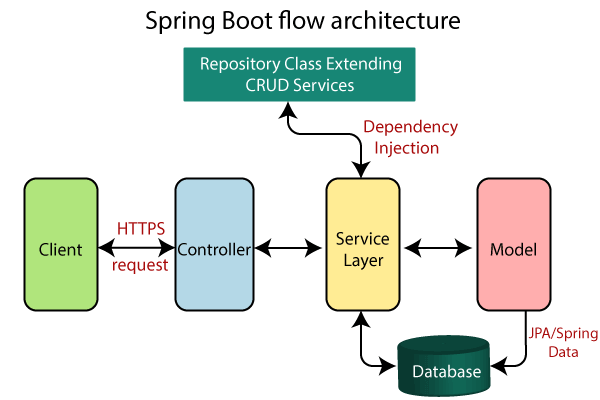
\includegraphics[width=0.8\textwidth, center]{spring-boot-architecture.png}
	\caption{Arhitectura de flux a Spring Boot}
\end{figure}

Clientul efectuează un request HTTP care este gestionat în primă instanță de \textbf{controller} care utilizează \textbf{servicii} necesare tratării request-ului. În acestea are loc logica operațiilor asupra înregistrărilor din baza de date cu ajutorul claselor \textbf{model} și prin intermediul unor clase \textbf{repository}. Informația de la client și către acesta are loc de cele mai multe ori sub forma unor obiecte DTO (Data Transfer Object) cinvertite în JSON în body-ul request-ului. Un exemplu de clasă DTO este cea a propunerilor, \texttt{ProposalDto}, ce conține strict informațiile de interes.

\begin{figure}[H]
	\centering
	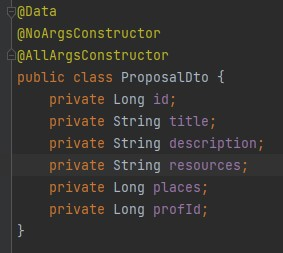
\includegraphics[width=0.4\textwidth, center]{proposaldto-class.jpg}
	\caption{Clasa ProposalDto}
\end{figure}

Aplicația de back-end poate fi considerată un \textit{REST API}. Un API este un set de definiții și protocoale pentru dezvoltarea unei aplicații de software, constituind în fapt un mediator între utilizator (în cazul de fată fiind aplicația de front-end) și resursele sau serviciile cerute într-un mod controlat și sigur \cite{rest-api}. REST (Representational State Transfer) este la rândul său un set de constrângeri arhitecturale ce trebuie respectate pentru ca un API să poată fi considerat RESTful.

Un astfel de API trebuie să urmeză în primul rând o arhitectură client-server, unde request-urile sunt gestionate prin intermediul protocolului HTTP. API-ul transferă o reprezentare a instanței unei resurse spre un anumit \textit{endpoint} (acesta include o adresă URL și identifică un canal de comunicare a resursei dintre back-end și front-end \cite{api-endpoint}), în format JSON de cele mai multe ori. De asemenea, această comunicare trebuie să fie \textit{stateless}, adică fiecare request este separat de restul și nu sunt reținute informații referitor la tranzacțiile anterioare. În al doilea rând, transferul de resurse este standardizat în ideea că acestea sunt separate de reprezentările trimise către client și manipulate de către acesta tot prin intermediul reprezentărilor \cite{rest-api}.

\section{Modelele}

Pentru a simula înregistrările dintr-o bază de date, Spring Boot dispune de posibilitatea de a defini clase ce identifică anumite entități cu ajutorul unor adnotări specifice. Spring Boot utilizează \textit{Entity Scanning} pentru a le identifica în loc de un fișier special cum ar fi \texttt{persistence.xml} în Spring. Clasele luate în considerare sunt cele adnotate cu \texttt{Entity}, \texttt{Embeddable} sau \texttt{MappedSuperclass} \cite{spring-boot-docs}.

Se observă de exemplu clasa \texttt{User}.

\begin{figure}[H]
	\centering
	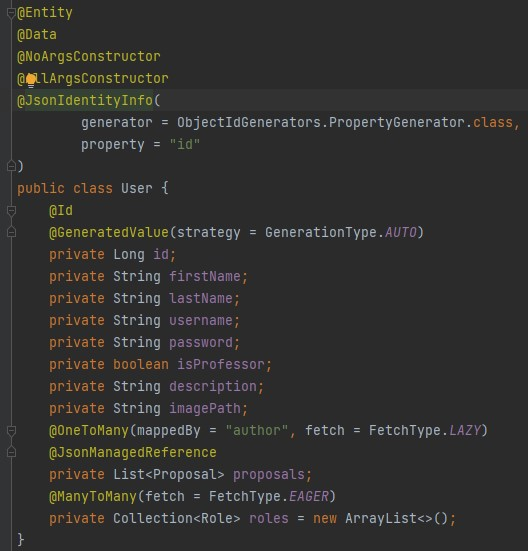
\includegraphics[width=0.6\textwidth, center]{user-class.jpg}
	\caption{Clasa User}
\end{figure}

Proprietățile acestei clase identifică câmpurile, identificate de numele lor, ale tabelei \texttt{user} din baza de date, iar tipul lor este conform reprezentării lor. Id-ul este generat automat cu ajutorul unei valori reținute în tabela \texttt{hibernate\_sequence} creată de framework-ul Hibernate, fiind de asemenea adnotată cu \texttt{@Id} pentru a sublinia că această proprietate reprezintă cheie primară.

Un utilizator de tipul profesor are o listă de propuneri (proposals, care sunt proiecte ori tematici), relația dintre tabela \texttt{user} și \texttt{proposal} prin intermediul cheilor străine (foregin keys) fiind specificată prin adnotarea \texttt{@OneToMany}. Opțiunea de \texttt{FetchType.LAZY} permite încărcarea mai rapidă a utilizatorului deoarece propunerile sale sunt instanțiate numai în cazul în care este nevoie. Fiecare utilizator are de altfel o colecție de roluri care pot fi \texttt{ROLE\_USER} în mod normal sau \texttt{ROLE\_ADMIN} și indică drepturile sale în aplicație.

Există și situația ca id-ul unei entități, precum cea a acordului, să fie compus, deoarece la nivelul reprezentării în tabela \texttt{accord}, o înregistrare este identificată prin id-urile studentului și profesorului care au hotărât colaborarea în realizarea unui anumit proiect. În consecință, a fost necesară crearea unei noi clase \texttt{AccordKey} care să simuleze cheia primară compusă și adnotarea proprietății cu \texttt{@EmbeddedId}.

\section{Clasele \textit{repository}}

Pentru fiecare entitate modelată în cadrul aplicației există o clasă \textit{repository} care reprezintă un mecanism de stocare, căutare și modificare a informațiilor din baza de date. Aceasta implementează interfața generică \texttt{JpaRepository} (Java Persistence API) care furnizeză o serie de metode CRUD (Create Read Update Delete) pentru accesarea datelor. Există posibilitatea de definirea a unor metode particulare prin cuvinte cheie care ajută la generarea automată a interogărilor SQL, fiind un mod clar și facil de efectuare a operațiilor \cite{jpa-repository}. Astfel de clase descriu nivelul de acces al datelor (Data Acces Layer)

\begin{figure}[H]
	\centering
	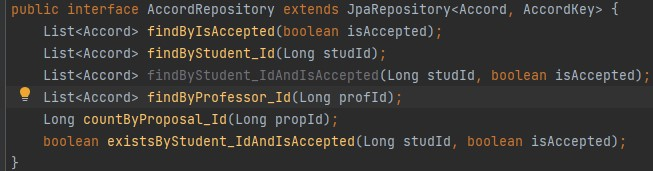
\includegraphics[width=0.8\textwidth, center]{accord-repository.jpg}
	\caption{Repository pentru un acord}
\end{figure}

Clasa \texttt{AccordRepository} conține de exemplu patru metode de căutare a acordurilor, în funcție de diferiți parametri. Metodele pot returna și dacă există o numită înregistrare, precum și numărul de anumite înregistrări. Datele sunt salvate sau actualizate cu metoda \texttt{save} ce primește ca argument un obiect entitate, în cazul în care id-ul este null, este introdusă o nouă înregistrare, altfel este modificată cea cu id-ul respectiv.

\section{Serviciile}

Aplicația dispune pentru entități de interfețe servicii corespunzătoare ce descriu metode de manipulare a datelor respective, implementate mai departe de clase ce trebuie adnotate cu \texttt{@Service} și care crează funcționalitățile necesare, reprezintă astfel teoretic nivelul serviciilor.

Serviciile utilizează clase \textit{repository} după cum este prezentat în figura următoare.

\begin{figure}[H]
	\centering
	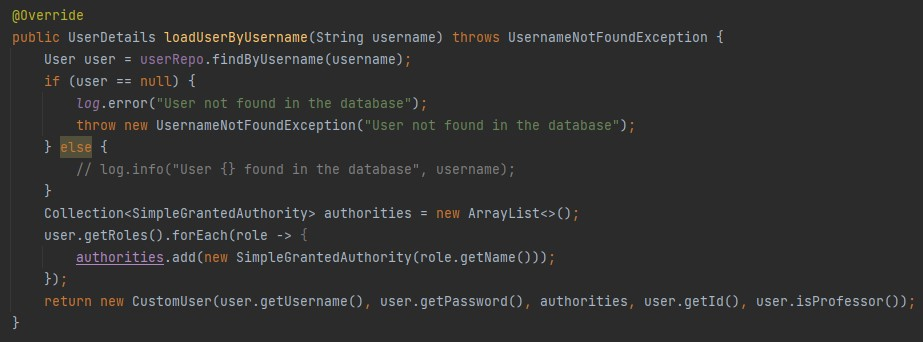
\includegraphics[width=0.8\textwidth, center]{user-service-load-method.jpg}
	\caption{Metodă de obținere a utilizatorului după username}
\end{figure}

Aceasta obține un obiect de tipul \texttt{User} cu un username dat și în plus rolurile acestuia, fiind convertit ulterior în \texttt{CustomUser} pentru verificarea și autorizarea utilizatorului autentificat în contextul aplicației.

\section{Controlerele (Controllers)}

Într-un final, cel de-al treilea nivel, de prezentare (presentation layer), este constituit de controlere care efectuează comunicarea cu partea de front-end și ale căror clase sunt adnotate cu \texttt{RestController}. Metodele descriu tratarea request-urilor HTTP cu ajutorul diferitelor servicii.

\begin{figure}[H]
	\centering
	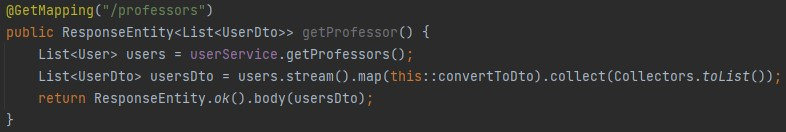
\includegraphics[width=1\textwidth, center]{user-controller-get-method.jpg}
	\caption{Metodă de trimitere a tuturor profesorilor}
\end{figure}

\begin{figure}[H]
	\centering
	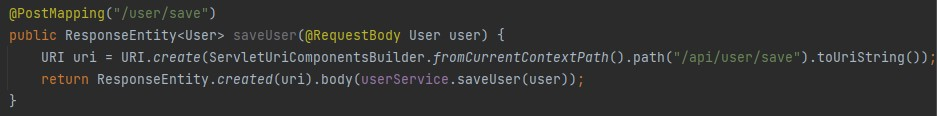
\includegraphics[width=1\textwidth, center]{user-controller-post-method.jpg}
	\caption{Metodă de salvare a unui utilizator}
\end{figure}

În cazul clasei \texttt{UserController}, metoda \texttt{getProfessors} este apelată de fiecare dată când este primit un request de tipul GET la endpoint-ul \texttt{"/professors"}, lucru evidențiat de adnotarea premergătoare definiției. Răspunsul HTTP este reprezentat de un obiect de tipul \texttt{ResponseEntity} cu \textit{status code} 200 (cerere efectuată cu succes) și având în \textit{body} o listă de obiecte de tipul \texttt{UserDto}, după cum a fost precizat anterior.

Metoda \texttt{saveUser} primește ca parametru un utilizator transmis prin body-ul request-ului POST, lucru ce trebuie specificat prin adnotarea \texttt{@RequestBody}.

\section{Securitatea}

Securitatea aplicației este dezvoltată de pachetul \texttt{security} care conține în principal clasa \texttt{SecurityConfig} ce extinde clasa abstractă \texttt{WebSecurityConfigurerAdapter} și este adnotată cu \texttt{Configuration} și \texttt{EnableWebSecurity}. Aceasta suprascrie metoda \texttt{configure} care indică maniera de tratare a utilizatorului ce interacționează cu aplicația.

\begin{figure}[H]
	\centering
	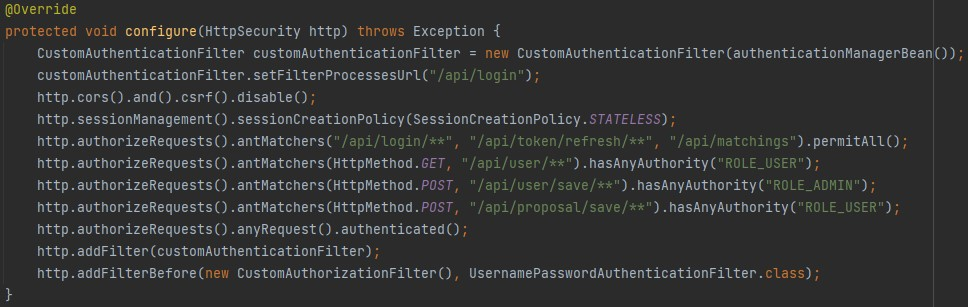
\includegraphics[width=1\textwidth, center]{security-configure-method.jpg}
	\caption{Metodă de configurare a securității}
\end{figure}

Metoda primește ca parametru o variabilă \texttt{http} de tipul \texttt{HttpSecurity} și care permite configurarea contextului abordat. Utilizând un sistem bazat pe chei JWT (JSON Web Token), aplicația de back-end nu trebuie să creeze o sesiune pentru fiecare utilizator.

JWT este un standard care definește un mod compact de trasmitere sigură a informațiilor între aplicații sub forma unor obiecte JSON, putând fi considerată o semnătură digitală a utilizatorului. Un astfel de token are trei părți separate de punct: header, payload și semnătură. Header-ul conține tipul token-ului, adică JWT, și algoritmul folosit pentru semnarea acestuia, aplicația \thesistitle utilizează \textit{HMAC256}. Payload-ul conține pretențiile (claims) cum ar fi rolurile deținute, dacă utilizatorul este profesor sau nu și altele. Semnătura este obținută prin criptarea primelor două părți cu algoritmul specificat și un șir de caractere secret știut doar de către back-end \cite{jwt}. Fiecare token are un termen de validitate pentru a indica perioada în care utilizatorul este autentificat.

De asemenea, request-urile din partea clientului sunt autorizate în funcție de anumite filtre, implementându-se în acest scop unul pentru autentificare în primă instanță și unul pentru autorizare.

\subsection{Autentificarea}

Autentificarea este verificarea identității unui utilizator, în acest caz find realizată într-un mod clasic cu ajutorul username-ului și parolei. Utilizatorul furnizeză credențialele sale care sunt verificate pe partea de back-end și sunt luate măsuri în funcție de validitatea acestora \cite{spring-security}.

Verificarea este asigurată de un filtru de autentificare.

\begin{figure}[H]
	\centering
	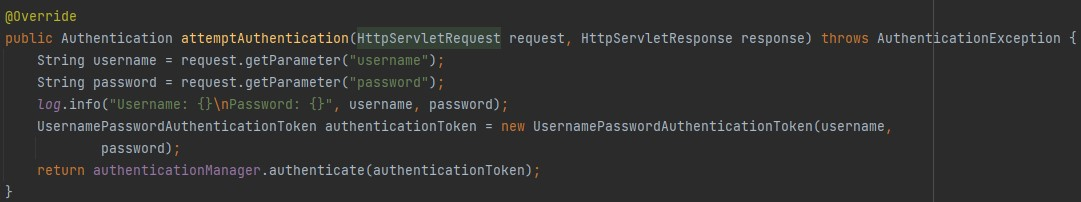
\includegraphics[width=1\textwidth, center]{attempt-authentication-method.jpg}
	\caption{Tentativă de autentificare}
\end{figure}

Atunci când un utilizator dorește acces la aplicație, în metoda descrisă mai sus este informată proporietatea \texttt{authenticationManager} de datele utilizatorului și încercă autentificarea acestuia.

\begin{figure}[H]
	\centering
	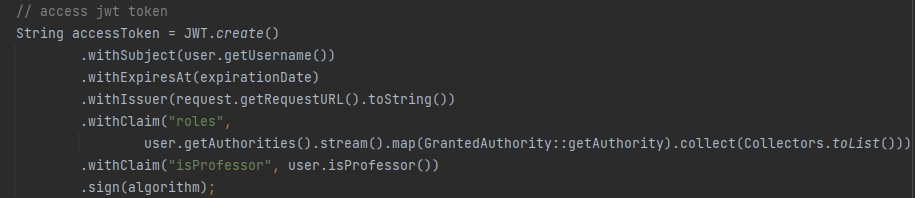
\includegraphics[width=1\textwidth, center]{successful-authentication-method-snippet.jpg}
	\caption{Autentificare cu succes}
\end{figure}

În cazul în care este autentificat cu succes, este creată cheia de acces, denumită \texttt{accessToken}, în metoda suprascrisă \texttt{successfulAuthentication}. Token-ul va conține informații despre username-ul persoanei, termenul de valabilitate, rolurile și tipul acesteia. Rezultatul este trimis către client sub formă de JSON. Această cheie JWT va fi folosită în toate request-urile viitoare ale utilizatorului pentru confirmare identității acesteia.

\subsection{Autorizarea}

Autorizarea este deciderea dacă o anumită persoană are permisiunea de a accesa o anumită resursă și este realizată în funcție de rolurile acesteia. Un administrator va avea de aceea un număr extins de drepturi cum ar fi adăugarea unui nou utilizator, acțiune pe care un cont doar cu ROLE\_USER nu o poate face. Modalitatea de autorizarea este restricționarea anumitor URL-uri în funcție de permisiuni \cite{spring-security}.

În consecință, fiecare utilizator este obligat ca, odată ce este autentificat, să poată fi identificat și autorizat înaintea de executarea request-urilor efectuate. După autentificarea cu succes a sa, utilizatorul primește un JWT (JSON Web Token), un șir de caractere ce conține criptat informații specifice cum ar fi username-ul, tipul de utilizator (profesor sau student) și permisiunile sale (ROLE\_USER, ROLE\_ADMIN).

\begin{figure}[H]
	\centering
	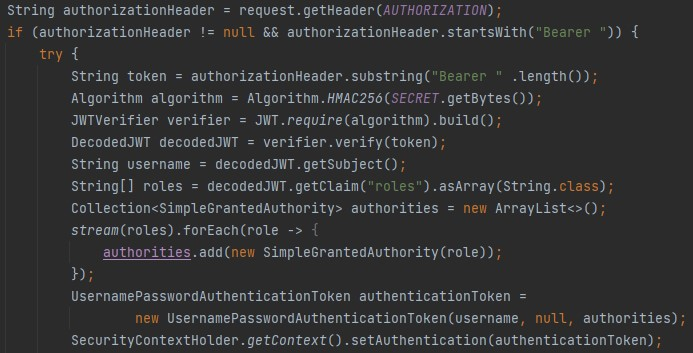
\includegraphics[width=1\textwidth, center]{authorization-filter-snippet.jpg}
	\caption{Autorizarea în \texttt{CustomAuthorizationFilter}}
\end{figure}

În filtrul de autorizare, este verificată validitatea requset-ului primit. Acesta trebuie să conțină un header \textit{Authorization} cu valoarea token-ului unic precedat de șirul de caractere "Bearer ". Cheia JWT este decriptată și este decisă acordarea permisiunii pentru reqest-ul respectiv. Dacă nu sunt îndeplinite condițiile adecvate, este trimis un răspun cu status code 401, \textit{Unauthorized}, sau 403, \textit{Forbidden}.
\\~\\
\indent După definirea celor două filtre cu responsabilitățile specifice, acestea sunt ordonate în mod logic pantru verificarea datelor și sunt descrise condițiile de validitate pentru rutele corespunzătoare request-urilor.

Există pe lângă cele două mecanisme menționate anterior un filtru care gestionează verificările CORS (Cross-Origin Resource Sharing) în care este specificată adresa de origine a aplicației de front-end, a clientului. Server-ul primește din partea browser-ului înainte de procesarea fiecărui request un \textit{preflight request} care verifică permisiunile pentru anumite metode HTTP. În consecință, metoda @Bean \texttt{corsConfigurationSource} din clasa \texttt{SecurityConfig} marchează adresa de origine \texttt{\url{http://localhost:4200}} a front-end-ului ca fiind de încredere și permite efectuarea request-urilor provenind de la acesta.